\documentclass[a4paper,12pt,oneside, tikz]{book}  
\usepackage[utf8]{inputenc}
\usepackage{tcolorbox}
\usepackage{amsmath,amssymb,amsthm, enumitem, hyperref, tabto} 
\usepackage[T1]{fontenc}
\usepackage[utf8]{inputenc}
\usepackage[english]{babel}
\usepackage{wrapfig}
\usepackage{lastpage}
\usepackage{tikz}
\usetikzlibrary{external}
\tikzexternalize % activate!
\usepackage[american]{circuitikz}
\usepackage[absolute,overlay]{textpos}
\usepackage[left=2cm,right=2cm]{geometry}
\usepackage[english]{babel}
\usepackage{fancyhdr}
\usepackage{float}
\hypersetup{
    colorlinks=true,
    linkcolor=blue,
    filecolor=magenta,      
    urlcolor=cyan,
    pdftitle={Studio 4},
    pdfpagemode=FullScreen,
    }

\urlstyle{same}
\usepackage{xcolor}
\usepackage{colortbl}

\usepackage{graphicx, multicol, latexsym}
\usepackage{blindtext}
\usepackage{subfigure}
\usepackage{caption}
\usepackage{capt-of}
\usepackage{tabu}
\usepackage{booktabs}

\usepackage{array}
\newcolumntype{P}[1]{>{\centering\arraybackslash}p{#1}}

\addto\captionsenglish{\renewcommand{\chaptername}{Activity}} 


\title{\textbf{Capacitors} Studio Report \\ CG1111A Studio 4}

\author{Prannaya Gupta (B02)}

\begin{document}

\maketitle

\chapter{The Energy Storage Capacity of Capacitors}

\section{Guidelines and Precautions}

\begin{itemize}
    \item Electrolytic and super capacitors have polarity. I will ensure that the polarities are
    correct before turning on the power supply.
    \item I will wear protective goggles when the electrolytic capacitors are powered.
\end{itemize}

\section{Set-Up}
\begin{figure}[H]
    \centering
    \subfigure[The Given Set-Up (C may represent alternative configurations)]{
        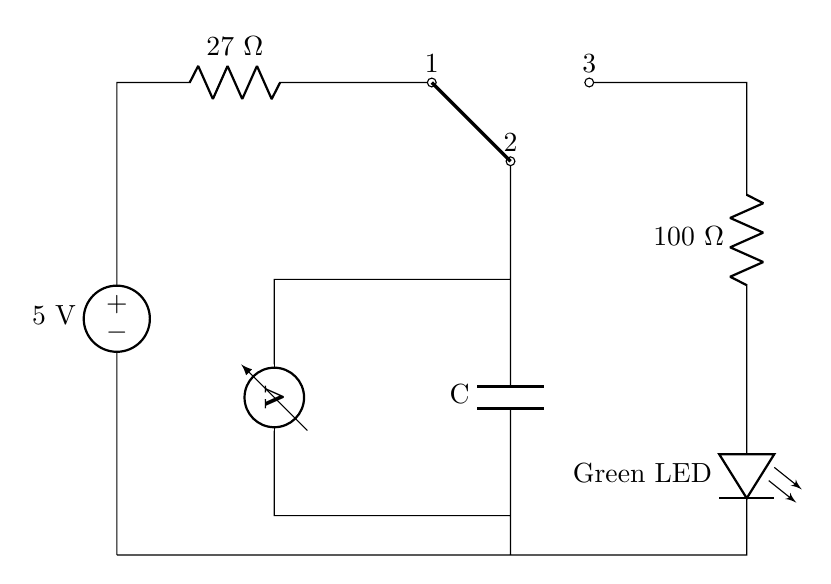
\begin{tikzpicture}[american voltages]
            \draw
              (6,6) to [short, o-] (8, 6)
              to [R, l_=100 $\Omega$] (8, 2)
              to [empty led, l_=Green LED] (8, 0)
              to [short, -] (0, 0)
              (5, 5) to[short, o-] (5, 4)
              to[C, l_=C] (5, 0)
              (4, 6) to[short, o-] (3,6)
              to [R, l_=27 $\Omega$] (0, 6)
              to [V, l_=5 V] (0, 0)
              (5, 0.5) to [short, -] (2, 0.5)
              to [voltmeter] (2, 3.5)
              to [short, -] (5, 3.5)
              (6, 6) node[above] {3}
              (5, 5) node[above] {2}
              (4, 6) node[above] {1};
              \draw[ very thick](5,5)--(4,6);
        \end{tikzpicture}
    }
    \subfigure[Breadboard Used]{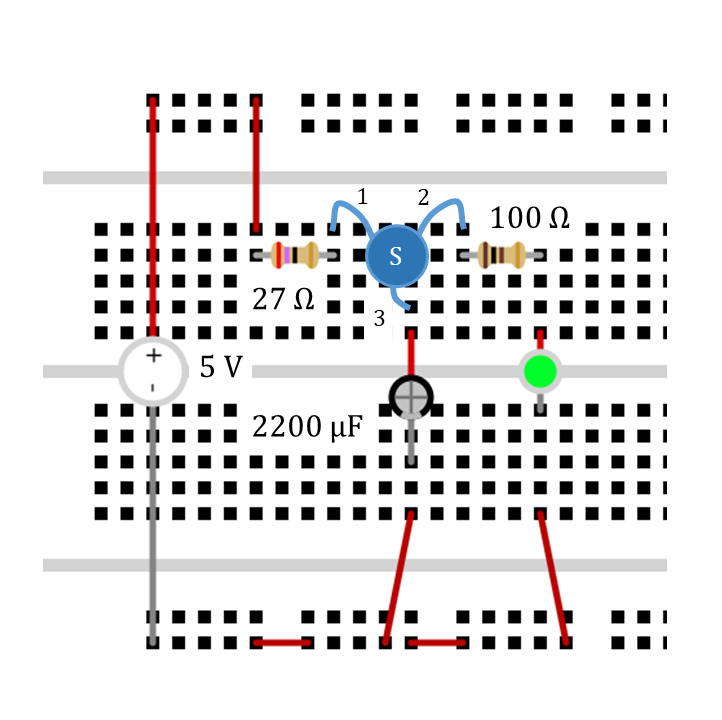
\includegraphics[width=0.5\textwidth]{images/breadboard1.png}}\label{fig:breadboard}
    
    \caption{Set-Up Planned} \label{fig:1}
\end{figure}

\section{Prepatory Calculations}

\begin{tcolorbox}
    \textbf{Calculate the peak charging current for the capacitor.} \\
    \\
    We know that for a charging capacitor,
    $$V = 5(1 - e^{-t/RC})$$
    Thus, we know that the current can be expressed as:
    $$I = \frac{dQ}{dt} = \frac{d}{dt} \left(CV \right) = \frac{5}{R} e^{-t/RC}$$

    This is still timebased, as we know that the maximum value for the exponential expresion for any non-negative value of $t$ is 1. Thus, we have that the peak charging current is:
    $$I_\text{peak} = \frac{5}{27} = 0.18519 \approx \textbf{0.185 A}$$

    This value is within the typical current supported by the USB cables in Laptops and Desktops (500 mA).
\end{tcolorbox}

\section{Results}
\begin{table}[H]
    \centering
    \begin{tabular}{|P{70mm}|P{40mm}|}
        \hline Capacitor C & Duration that the LED lights up (s) \\
        \hline Single 2200 $\mu$F capacitor & 1.17  \\
        \hline Two 2200 $\mu$F capacitors in \textbf{parallel} & 2.35 \\
        \hline Single 1 F supercapacitor & > 1 min \\
        \hline 1 F supercapacitor in \textbf{series} with a 2200 $\mu$F capacitor & 1.85 \\
        \hline
    \end{tabular}
    \caption{Table of Final Values}
    \label{tab:final}
\end{table}

\section{Discussion}
\begin{tcolorbox}
    \textbf{Calculate energy stored in each capacitor and justify the time that the LED lights up for.} \\
    \\

    For set-up 1, the effective capacitance is given by:
    $$C_eff = C = \text{2200 }\mu\text{F}$$
    Thus, the energy in the capacitor "C" in set-up 1 is given by:
    $$E_1 = E_{2,1} = E_{2,2} = \frac{1}{2}CV^2 = \frac{1}{2} (2200 \times 10^{-6})(5)^2 = \textbf{0.0275 J}$$

    For set-up 2, the effective capacitance is given by:
    $$C_eff = C_1 + C_2 = 2\times 2200 = \text{4400 }\mu\text{F}$$
    Thus, the energy in the capacitor "C" in set-up 2 is given by:
    $$E_2 = \frac{1}{2}CV^2 = \frac{1}{2} (4400 \times 10^{-6})(5)^2 = \textbf{0.055 J}$$

    For set-up 3, the effective capacitance is given by:
    $$C_eff = C = \text{1 F}$$
    Thus, the energy in the capacitor "C" in set-up 3 is given by:
    $$E_3 = \frac{1}{2}CV^2 = \frac{1}{2} (1)(5)^2 = \textbf{12.5 J}$$

    For set-up 4, the effective capacitance is given by:
    $$C_eff = \left(\frac{1}{C_1} + \frac{1}{C_2}\right)^{-1} = \left(\frac{1}{2200 \times 10^{-6}} + \frac{1}{1}\right)^{-1} = 0.0021952\text{ F} \approx \text{2200 }\mu\text{F}$$
    Thus, the energy in the capacitor "C" in set-up 4 is given by:
    $$E_1 = E_{2,1} = E_{2,2} = \frac{1}{2}CV^2 = \frac{1}{2} (2200 \times 10^{-6})(5)^2 = \textbf{0.0275 J}$$

    Since the energy in set-up 2 is twice than in set-up 1, it makes sense why, in the same set-up where a similar amount of power was dissipated in the resistive element, set-up 2's LED lasted for about twice as long as that in set-up 1.

    Meanwhile, since the energy in set-up is significantly is larger, it also justifies the excessive time taken for it to surpass the forward current for the similarly structured circuit as in set-up 1.

    Set-up 4 is about the same in terms of energy to set-up 1, which represents that it's power dissipation is also similar.
\end{tcolorbox}

\chapter{The Charging Voltage of Capacitors}
\section{Set-Up}

\begin{figure}[htbp]
    \centering
    \subfigure[The Given Set-Up]{
        \begin{tikzpicture}
            \draw
              (0, 0) to [short, -o] (6, 0) node[below]{b}
              to [short, -] (6, 1)
              to [C, l_=2200 $\mu$F, v_=] (6,3)
              to [short, -o] (6, 4) node[above]{a}
              to [short, -] (4, 4)
              to [R, l_=180 $\Omega$] (0, 4)
              to [short, -o] (0, 3.5)
              (0, 2.5) to[short, o-] (0, 2)
              to[V, l_=5 V] (0, 0)
              to [short, -] (4, 0)
              to [R, l_=180 $\Omega$] (4, 4);
              \draw[ very thick](0,2.5)--(-0.5,3.5);
        \end{tikzpicture}
    }
    \subfigure[Breadboard Used]{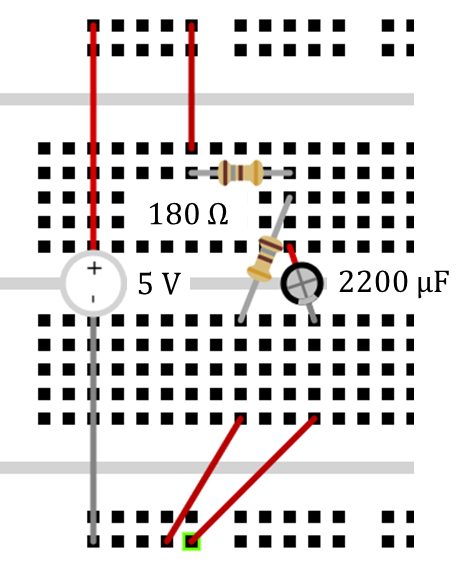
\includegraphics[width=0.3\textwidth]{images/breadboard2.png}}\label{fig:breadboard2}
    
    \caption{Set-Up Planned} \label{fig:2}
\end{figure}

\section{Preparatory Calculations}
\subsection{Preliminaries}
\begin{tcolorbox}
    Fill in the values for the following questions:
    \begin{enumerate}
        \item The voltage across the capacitor just before the switch is closed, $v_c(0^-) = $\textbf{ 0 V}.
        \item The voltage across the capacitor just after the switch is closed, $v_c(0^+) = $\textbf{ 0 V}.
        \item The expected voltage at steady-state long after the switch is closed, $v_c(\infty) = $\textbf{ 5 V}.
    \end{enumerate}
    
\end{tcolorbox}

\section{Thevenin Equivalent Circuit}

\begin{figure}[H]
    \centering
    \subfigure[The Thevenin Voltage Load]{
        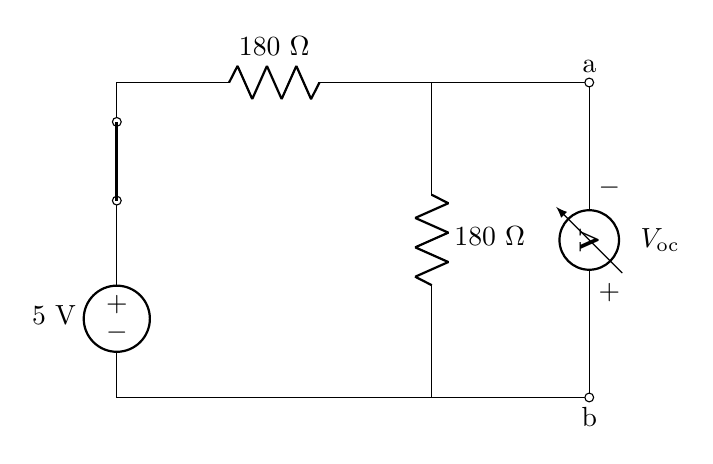
\begin{tikzpicture}
            \draw
              (0, 0) to [short, -o] (6, 0) node[below]{b}
              to [short, -] (6, 1)
              to [voltmeter, v_=$V_\text{oc}$] (6,3)
              to [short, -o] (6, 4) node[above]{a}
              to [short, -] (4, 4)
              to [R, l_=180 $\Omega$] (0, 4)
              to [short, -o] (0, 3.5)
              (0, 2.5) to[short, o-] (0, 2)
              to[V, l_=5 V] (0, 0)
              to [short, -] (4, 0)
              to [R, l_=180 $\Omega$] (4, 4);
              \draw[ very thick](0,2.5)--(0,3.5);
        \end{tikzpicture}
    }
    \subfigure[The Thevenin Current Load]{
        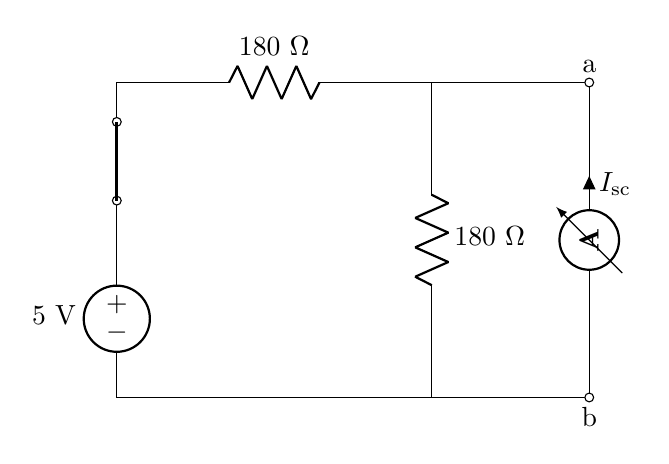
\begin{tikzpicture}
            \draw
              (0, 0) to [short, -o] (6, 0) node[below]{b}
              to [short, -] (6, 1)
              to [ammeter, i_=$I_\text{sc}$] (6,3)
              to [short, -o] (6, 4) node[above]{a}
              to [short, -] (4, 4)
              to [R, l_=180 $\Omega$] (0, 4)
              to [short, -o] (0, 3.5)
              (0, 2.5) to[short, o-] (0, 2)
              to[V, l_=5 V] (0, 0)
              to [short, -] (4, 0)
              to [R, l_=180 $\Omega$] (4, 4);
              \draw[ very thick](0,2.5)--(0,3.5);
        \end{tikzpicture}
    }
    \caption{Thevenin Computational Circuits}
    \label{fig:thevenin}

\end{figure}


As seen from Figure \ref{fig:thevenin}, we know that $V_\text{oc}$ is simply the potential difference across one of the two 180 $\Omega$ resistors, while $I_\text{sc}$ is the short circuit current.

To derive $V_\text{oc}$:
\begin{align*}
    V_\text{oc} &= V_{\text{180} \Omega} \\
    &= \varepsilon \times \frac{180}{180+180} \text{\quad (KVL)} \\
    &= 5 \times \frac{1}{2} = \textbf{2.5 V}
\end{align*}

To derive $I_\text{sc}$ and thus $R_\text{th}$:
\begin{align*}
    I_\text{sc} &= \frac{\varepsilon}{R_\text{eff}} \\
    &= \frac{5}{180} \text{\quad (Since it short-circuits)} \\
    &= \frac{1}{36} \\
    R_\text{th} &= \frac{V_\text{oc}}{I_\text{sc}} \\
    &= 2.5 \times 36 = \textbf{90 }\bf{\Omega}
\end{align*}

Thus we can redraw the circuit as shown in Figure \ref{fig:thevenin}.

\begin{figure}[H]
    \centering
    \begin{tikzpicture}
        \draw
            (0, 0) to [short, -] (4, 0)
            to[C, l_=2200 $\mu$F] (4, 4)
            to[R, l_=90 $\Omega$] (0, 4)
            to[short, -o] (0, 3.5)
            (0, 2.5) to[short, o-] (0, 2)
            to[V, l_=2.5 V] (0, 0);
            \draw[ very thick](0,2.5)--(0,3.5);
    \end{tikzpicture}
    \caption{Thevenin Equivalent Circuit}
    \label{fig:theveninEq}

\end{figure}


The expression for the transient voltage is:
$$v_c(t) = 0(e^{-t/0.198}) + 2.5(1 - e^{-t/0.198})$$

\newpage
\section{Results}

\begin{figure}[ht]
    \centering
    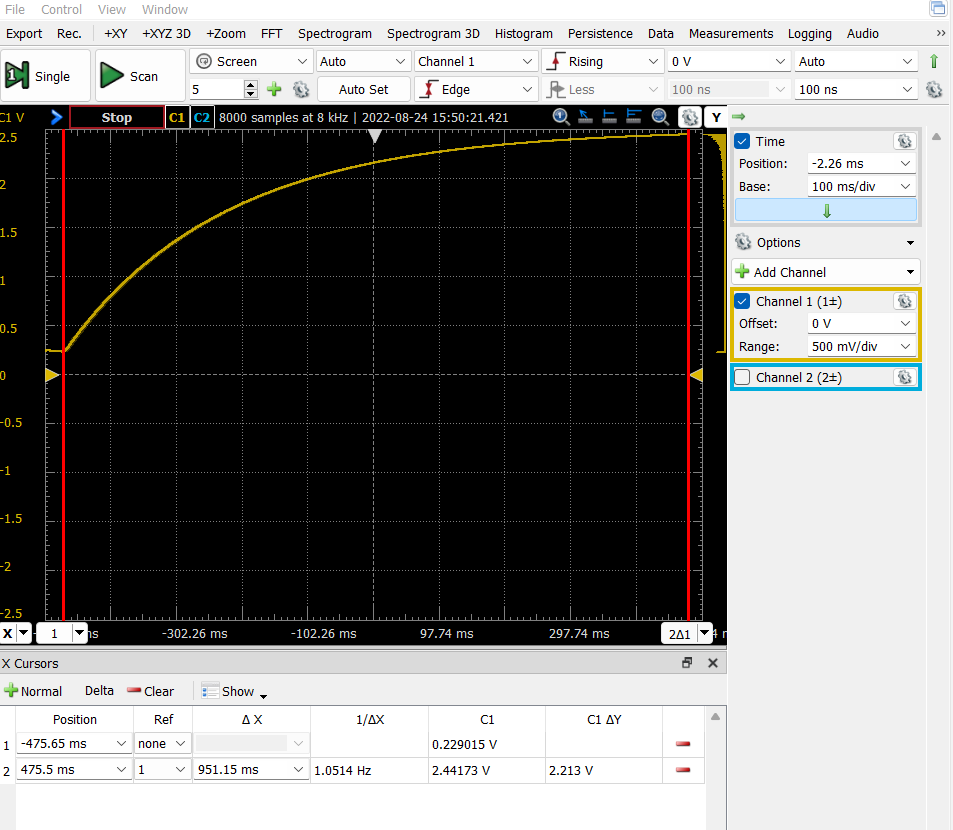
\includegraphics[width=1\textwidth]{images/activity2result.png}
    \caption{Final Result}
    \label{fig:result}
\end{figure}

Final Results:
\begin{itemize}
\item $\Delta$ X = 0.189 ms
\end{itemize}

\begin{tcolorbox}
Based on the equation you have written in Step 4, what is the theoretical value of this time (i.e., the time taken for the capacitor’s voltage to reach 63.2\% of $v_c(t = \infty)$)?


\begin{align*}
v_c(t) &= 2.5(1 - e^{-t/0.198)}) \\
\frac{v_c(t)}{2.5} &= 1 - e^{-t/0.198} \\
1 - 0.632 &= e^{-t/0.198} \\
t/0.198 &= -\ln \left(0.368 \right) \\
t &= -0.198\ln \left(0.368 \right) \\
&\approx \textbf{0.198 s}
\end{align*}

This is slightly larger than the measured value, but it is effectively the same theoretically and experimentally.
\end{tcolorbox}

\begin{tcolorbox}
Give two possible sources of errors.
\begin{itemize}
    \item Voltmeter is not ideal, so there is some current flowing into the voltmeter which could affect our final results.
    \item Wires are not of zero resistance, hence there may be some resistance that is left unaccounted for.
\end{itemize}
\end{tcolorbox}
\end{document}
